% Public explainer for toolcall-contract, written for a non-specialist
% reader. Every number and every quoted tool call is taken from the
% committed datasets in this repository; the figure is the one rendered
% by tools/render_figures.py from the same replay CI runs.
%
% Build from this directory:  latexmk -pdf explainer.tex
%
% When the datasets change, the counts in "What two models actually did"
% and the quoted calls must be re-checked against reports/ and
% tools/inspect_failures.py. They are prose, so nothing enforces them.
\documentclass[11pt,a4paper]{article}

\usepackage[margin=2.4cm,top=2.2cm,bottom=2.2cm]{geometry}
\usepackage[T1]{fontenc}
\usepackage[utf8]{inputenc}
\usepackage{lmodern}
\usepackage{microtype}
\usepackage{graphicx}
\usepackage{xcolor}
\usepackage{titlesec}
\usepackage{enumitem}
\usepackage[hidelinks]{hyperref}
\usepackage{fancyhdr}
\usepackage{tcolorbox}
\tcbuselibrary{skins,breakable}

\graphicspath{{../figures/}}

\definecolor{navy}{HTML}{0F2F52}
\definecolor{gold}{HTML}{B08D3F}
\definecolor{ink}{HTML}{1A1A1A}
\definecolor{soft}{HTML}{F7F5F0}
\definecolor{rule}{HTML}{D8D3C8}

\color{ink}
\linespread{1.09}
\setlength{\parskip}{6pt}
\setlength{\parindent}{0pt}

\titleformat{\section}{\large\bfseries\color{navy}}{}{0pt}{}
\titlespacing*{\section}{0pt}{16pt}{6pt}

\pagestyle{fancy}
\fancyhf{}
\renewcommand{\headrulewidth}{0pt}
\fancyfoot[C]{\small\color{gray}\thepage}

\newtcolorbox{quotebox}[1][]{
  enhanced, breakable, colback=soft, colframe=gold,
  boxrule=0pt, leftrule=2.5pt, arc=0pt, outer arc=0pt,
  left=10pt, right=10pt, top=8pt, bottom=8pt, #1}

\newcommand{\code}[1]{{\ttfamily\small #1}}

\begin{document}

\begin{center}
{\LARGE\bfseries\color{navy} Well-formed and wrong}\\[6pt]
{\large Why checking an AI's instructions against a schema is not enough}\\[12pt]
{\small Munawar Kazmi \;\textbullet\; \href{https://munawarkazmi.com}{munawarkazmi.com}}\\[2pt]
{\small A plain-language guide to \textbf{toolcall-contract}, an open validator for the commands language models send to real systems.}\\[2pt]
{\small Code, datasets, and every figure: \href{https://github.com/munawarkazmi/toolcall-contract}{github.com/munawarkazmi/toolcall-contract}}
\end{center}

\vspace{4pt}
{\color{rule}\hrule height 1pt}
\vspace{10pt}

\section{When an AI presses the buttons}

Modern AI assistants do not only write text. They operate things. When you ask an assistant to book a meeting, adjust a thermostat, or move a robot, the model does not touch the machinery directly. It fills in a form.

The form is called a tool call, and it looks like this:

\begin{quotebox}
\code{\{"tool": "navigate\_to\_waypoint", "arguments": \{"waypoint": "dock"\}\}}
\end{quotebox}

A name for the thing to do, and the values to do it with. Some other piece of software reads that form and actually drives the robot.

So the interesting question is not whether the model writes good prose. It is whether the form it filled in is one you would be happy to act on.

\section{Everyone checks the shape of the form}

There is a standard way to check these forms, and essentially every AI system that uses tools does it. It is called schema validation, and it asks structural questions:

\begin{itemize}[leftmargin=1.4em,itemsep=2pt]
\item Is this valid, parseable data at all?
\item Is \code{navigate\_to\_waypoint} a tool that actually exists?
\item Does it have the fields it is supposed to have, and are they the right types? A number where a number belongs, text where text belongs, nothing missing.
\end{itemize}

These checks are real and worth doing. They are also, it turns out, almost never the thing that goes wrong.

Consider this call, produced by a real model when asked to pick up a green cylinder:

\begin{quotebox}
\code{\{"tool": "pick\_object", "arguments": \{"object\_id": "green\_cylinder",}\\
\code{\hspace*{9.4em}"gripper\_force": 20\}\}}
\end{quotebox}

It parses. The tool exists. Every field is present and correctly typed. It passes schema validation completely.

There is no green cylinder. It is not in the robot's catalogue of objects and never was. The call is perfectly formed and refers to something that does not exist, and the check that most systems rely on has nothing to say about it, because ``does this thing exist?'' is not a question about shape.

\section{The second layer}

toolcall-contract is a validator with two layers. The first is the structural check just described. The second asks the questions a schema cannot:

\begin{itemize}[leftmargin=1.4em,itemsep=2pt]
\item \textbf{Does the thing referred to exist?} Waypoints, objects, people and zones are checked against the actual catalogues of what is out there.
\item \textbf{Do the numbers contradict each other?} A task that ends before it begins is well-typed and impossible.
\item \textbf{Are conditional requirements met?} If you say the setting applies to a zone, you have to name the zone.
\item \textbf{Are mutually exclusive options being combined?} Some settings cannot both be true.
\end{itemize}

The first layer is checked against an established, independent validation library across 25,000 randomly generated combinations of rules and data. The two agreed on all 25,000, with zero disagreements. That matters because the whole point of this project is the second layer, and a second layer built on a shaky first one would prove nothing.

\section{What two models actually did}

Forty tasks were put to two different language models, both with randomness switched off so the results reproduce exactly. One is small and runs on a laptop; the other is roughly ten times larger and runs in a data centre. Every response is committed to the repository.

Neither model invented a tool that did not exist. Neither model broke a single schema.

\begin{quotebox}
The structural layer alone, the check most systems stop at, would have passed 39 of the 40 calls. For both models. It caught almost nothing, because there was almost nothing of that kind to catch.
\end{quotebox}

The second layer caught seven bad calls from the smaller model and five from the larger one. Every one of them was a call that a schema check waves straight through.

\begin{figure}[t]
\centering
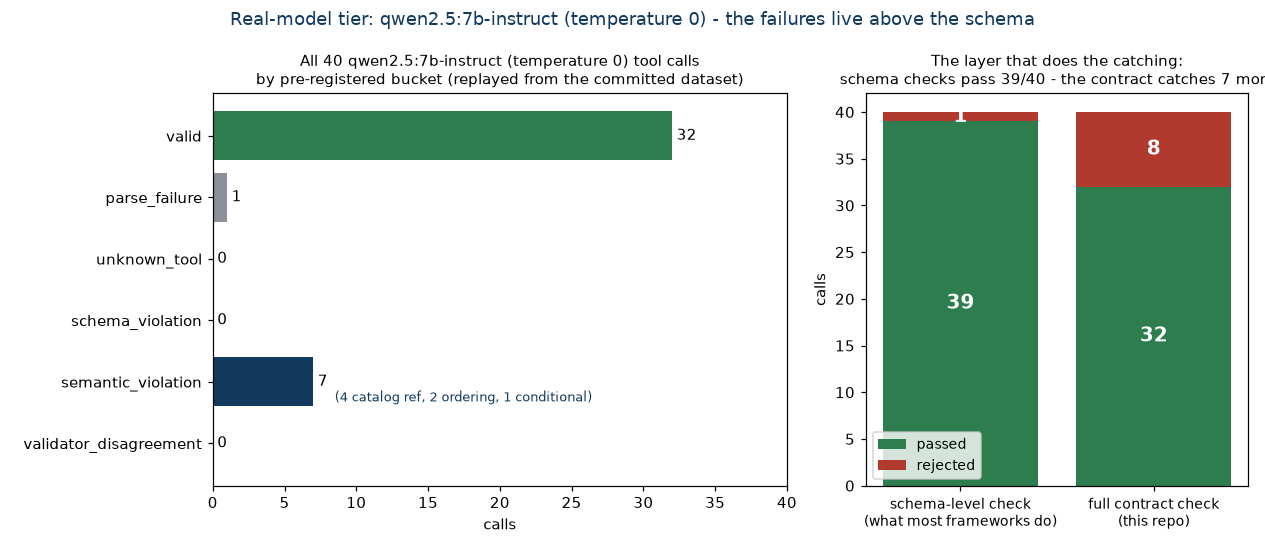
\includegraphics[width=\linewidth]{qwen_layers.png}
\caption{\small The smaller model's forty calls. On the left, where they land: no invented tools, no broken schemas, seven contract violations. On the right, the comparison that matters: a schema-level check passes 39 of 40, the full contract check rejects 8. The failures live above the schema.}
\end{figure}

\section{Three ways to be well-formed and wrong}

The failures fall into three families, and all of them are quoted here exactly as the model produced them.

\textbf{Faithfully writing down something that does not exist.} Asked to place a battery pack at the workbench, when no workbench exists:

\begin{quotebox}
\code{\{"tool": "place\_object", "arguments": \{"object\_id": "battery\_pack",}\\
\code{\hspace*{9.4em}"waypoint": "workbench"\}\}}
\end{quotebox}

The model is not being careless. It is being obedient. It was told about a workbench, so it wrote down a workbench. The same pattern produced calls referring to a nonexistent person, a nonexistent zone and a nonexistent object.

\textbf{Copying a contradiction without noticing it.} Asked to schedule a delivery starting at second 900 and ending at second 300:

\begin{quotebox}
\code{\{"tool": "schedule\_task", "arguments": \{"task\_type": "deliver",}\\
\code{\hspace*{9.4em}"start\_time": 900, "end\_time": 300\}\}}
\end{quotebox}

Both numbers are numbers, so the schema is satisfied. The delivery finishes ten minutes before it starts. The request itself was impossible, and the model transcribed the impossibility rather than flagging it. Another call set a boundary running from 9.0 down to 1.0, the same failure in a different costume.

\textbf{Leaving a requirement dangling.} Asked to set a speed limit for a zone without being told which zone:

\begin{quotebox}
\code{\{"tool": "set\_speed\_limit", "arguments": \{"limit": 1.5, "scope": "zone"\}\}}
\end{quotebox}

It says the limit applies to a zone, and never says which. Well-typed, and unactionable.

\section{The most honest thing either model did}

One task asked both models to rotate a camera. There is no camera tool.

The smaller model replied with an empty object, \code{\{\}}, effectively saying nothing at all. The larger one wrote a short refusal in plain prose naming the missing capability.

Neither invented a camera tool to look helpful. Both failures land in a bucket that exists specifically for this, and it is arguably the best behaviour in either dataset: when the right answer is ``I cannot do that with what I have'', saying nothing is far better than confidently pressing the wrong button.

\section{The line this validator will not pretend to cross}

Here is the part that matters most, and it is an admission rather than a result.

Several of the forty requests were impossible or wrong, and the models quietly turned them into something possible instead. Every one of these calls passes the contract check completely, and is counted as valid:

\begin{itemize}[leftmargin=1.4em,itemsep=2pt]
\item Asked to go to \emph{warehouse 3}, which does not exist, the model went to \code{storage\_a} instead. It did not ask, and it did not object.
\item Asked to set the speed limit to \emph{5 metres per second}, above what the system permits, it set \code{0.5}. Ten times slower than requested, silently.
\item Asked to \emph{turn the robot off}, which no tool can do, it sent back a battery status report.
\end{itemize}

Every one of those is a legal, well-formed, contract-satisfying call. The validator passes them, deliberately, and says so in public.

\begin{quotebox}
Whether a call does what the person actually meant is a different question from whether it is valid, and it needs different machinery. Merging the two into a single ``valid'' score would hide exactly these cases. This project declares that boundary up front rather than quietly scoring across it.
\end{quotebox}

That is an unusual thing for a piece of software to say about itself, and it is the reason the numbers above can be trusted: the tool reports what it can check, and names what it cannot.

\section{How it is kept honest}

The categories every call falls into were written down and committed before any results were published, so no flattering category could be invented after seeing the data. Two of those categories are load-bearing: the number of times the two structural checkers disagreed, and the number of times something invalid was marked valid. Both are zero, and the automated tests reject any change that makes them anything else.

Beyond the two models, 262 hand-built cases with known correct answers exercise every rule, and the validator must match every one exactly.

Reproducing all of it needs no AI model and no internet connection. Every response is committed, so the evaluation replays deterministically on any computer, and the tests do exactly that on every change.

\section{What this does not show}

Two models, at one setting each, on forty tasks apiece. That is a small sample and the counts are reported per model, never averaged into a claim about ``language models''. The tool catalogue is a robotics one, so the specific failures are robot-flavoured, though nothing about the three failure families is specific to robots.

The strongest available next step is more models and more tasks, to find out whether ``the failures live above the schema'' holds as broadly as these two suggest.

\section{Why it matters}

AI systems are increasingly wired to things that act: robots, databases, payment systems, calendars. The industry standard for checking those commands answers whether the message is shaped correctly.

On this evidence, shape was never the problem. Both models filled in the form perfectly every single time, and still produced commands that referred to objects that do not exist, scheduled deliveries that end before they begin, and set limits on unnamed zones. Those calls are what reaches the machinery, and a checker that only reads the shape will forward every one of them.

\vspace{6pt}
{\color{rule}\hrule height 1pt}
\vspace{6pt}

{\small Every task, every raw model response, every figure, and the validator itself are public. This guide is part of a wider line of work on machines that know their own limits: a benchmark measuring \emph{how} language model planners fail, a safety layer that detects unsafe robot routes and recovers or halts, and this validator, which checks the commands before they are sent.\\
Repository: \href{https://github.com/munawarkazmi/toolcall-contract}{github.com/munawarkazmi/toolcall-contract}}

\end{document}
